%% Preamble
\documentclass{beamer}
%\usetheme[beteckna]{Median}
\usepackage{euler}
\usepackage[T1]{fontenc}
\usepackage[black]{merriweather}
%\usepackage[eulergreek]{sansmath}
\usepackage{tikz}
\usepackage{wasysym}
\usetheme{Median}

%% Macros
\renewcommand{\l}{\lambda} % We don't really care about this diacritic
\newcommand{\lf}[2]{\lambda{#1}.\,{#2}}
\newcommand{\aeq}{=_{\alpha}}
\newcommand{\ato}{\to_{\alpha}}
\newcommand{\beq}{=_{\beta}}
\newcommand{\bto}{\to_{\beta}}
\newcommand{\apause}{\action<+->}
\newenvironment{blankframe}
{% This is entirely within local scope
    \setbeamertemplate{navigation symbols}{}
    \setbeamertemplate{background}{}
    \begin{frame}[plain]
}{%
    \end{frame}
}
\newcommand{\simpleimage}[1]{%
    \begin{tikzpicture}[remember picture,overlay]
        \node[at=(current page.center)] {%
            \includegraphics[height=0.95\paperheight]{#1}
        };
    \end{tikzpicture}
}

\newcommand{\TRUE}{\textsf{TRUE}}
\newcommand{\FALSE}{\textsf{FALSE}}
\newcommand{\AND}{\textsf{AND}}
\newcommand{\OR}{\textsf{OR}}
\newcommand{\NOT}{\textsf{NOT}}
\newcommand{\IF}{\textsf{IF}}

\newcommand{\PAIR}{\textsf{PAIR}}
\newcommand{\FIRST}{\textsf{FIRST}}
\newcommand{\SECOND}{\textsf{SECOND}}

\newcommand{\SUCC}{\textsf{SUCC}}
\newcommand{\PLUS}{\textsf{PLUS}}
\newcommand{\MULT}{\textsf{MULT}}
\newcommand{\EXP}{\textsf{EXP}}
\newcommand{\ISZERO}{\textsf{ISZERO}}
\newcommand{\PRED}{\textsf{PRED}}
\newcommand{\FACT}{\textsf{FACT}}

\newcommand{\CONS}{\textsf{CONS}}
\newcommand{\HEAD}{\textsf{HEAD}}
\newcommand{\TAIL}{\textsf{TAIL}}
\newcommand{\NIL}{\textsf{NIL}}
\newcommand{\ISNIL}{\textsf{ISNIL}}

\newcommand{\ID}{\textsf{ID}}
\newcommand{\Y}{\textbf{Y}}
\newdateformat{monthyear}{\shortmonthname[\THEMONTH] \THEYEAR}

%% Title and other silliness
\title{An Introduction to the $\l$-calculus}
\author{Toli Paine}
\institute{Quantcast}
\date{\monthyear\today}

\AtBeginSection {%
    \begin{frame}[plain]
        \frametitle{\\[2em]}
        \tableofcontents[currentsection]
    \end{frame}
}

% We're going to want this later
%\[
%    y \equiv \l f.(\l x.f (x x)) (\l x.f (x x))
%\]

%% Slides
\begin{document}
    \frame{\titlepage}

    \section{Introduction}
    \begin{frame}
        \frametitle{Why the $\l$-calculus?}
        \pause
        \begin{itemize}[<+->]
            \setlength{\itemsep}{1.5em}
            \item Simple, yet powerful: encompasses all of computing
                (Turing-complete!)
            \item Much easier to understand than Turing machines
            \item Provides the basis of all ``functional programming''
                languages \\[0.25em]
                \begin{itemize}[<+->]
                    \item Scala, Clojure, Scheme, Haskell
                \end{itemize}
                \vspace{-0.5em}
            \item Ever wonder what the hell ``Y Combinator'' actually means?
        \end{itemize}
    \end{frame}

    \section{Background}
    \begin{blankframe}
        \simpleimage{church.jpg}
    \end{blankframe}
    \begin{blankframe}
        \simpleimage{turing.jpg}
    \end{blankframe}
    \begin{blankframe}
        \vspace{-0.75em}
        \begin{center}
            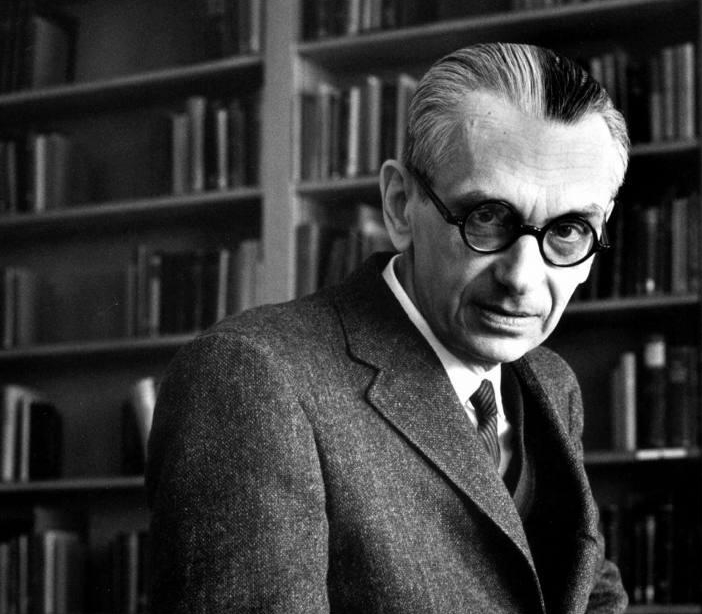
\includegraphics[height=0.8\paperheight]{godel-crop.jpg} \\
        \end{center}
        \vspace{-1em}
        \begin{quote}
            \hspace{2em}\textit{``Modern math's absolute Prince of Darkness''}
        \end{quote}
        \hspace{6em} {\footnotesize
            --- David Foster Wallace, \textit{Everything and More}
        }
    \end{blankframe}

    % TODO
    \begin{frame}
        \frametitle{The Church-Turing Thesis}
        \begin{align*}
            \hspace{-2em}
            \apause {%
                \parbox{0.6\paperwidth}{%
                    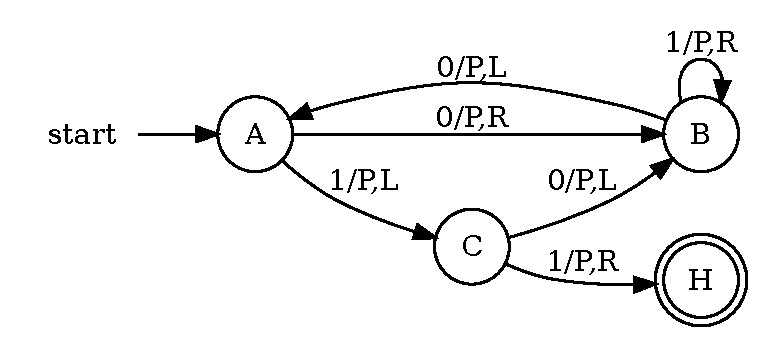
\includegraphics[width=0.55\paperwidth]{turing-machine.eps}
                }
            }
            \apause {&\scalebox{3}{$=$}}
            \apause {&\scalebox{5}{$\l$}}
        \end{align*}
    \end{frame}

    \begin{frame}
        \frametitle{Definitions: Syntax}
        \begin{itemize}[<+->]
            \item Variables: $v_0, \, v_1, \, v_2, \, \ldots, \, v_n, \, \ldots$ \\[1em]
            \item Abstraction using '$\l$' and '.' (right-binding):
                \begin{align*}
                    \ID   & \equiv \lf{x}{x} \\
                    \lf{x\,y}{x}        & \equiv \lf{x}{\lf{y}{x}}
                \end{align*}
            \item Application (left-binding):
                \begin{align*}
                    f \, x        & \to \textsf{``apply $f$ to $x$''} \\
                    f \, x \, y   & \to (f \, x) \, y
                \end{align*}
            \item Grouping using parens: $(\lf{x}{x})\, y \neq (\lf{x}{x \, y})$
        \end{itemize}
    \end{frame}

    \begin{frame}
        \frametitle{Definitions: Reduction and Equivalence}
        \begin{itemize}[<+->]
            \setlength{\itemsep}{1.5em}
            \item \textbf{$\alpha$-equivalence} is structural equality:
                \begin{align*}
                    \lf{x}{x}       &\aeq \lf{y}{y} \\
                    \lf{x\,y}{x}    &\aeq \lf{\smiley\,\frownie}{\smiley}
                \end{align*}
            \item \textbf{$\beta$-reduction} is function application:
                \[
                    (\lf{x}{x}) \, y \bto y
                \]
            \item And thus \textbf{$\beta$-equivalence} is ``computational''
                equality:
                \[
                    (\lf{x\,y}{x}) \, p \, q \beq (\lf{x}{x}) \, p \beq p
                \]
        \end{itemize}
    \end{frame}

    \section{Boolean Logic}
    \begin{frame}
        \frametitle{Encoding truth values}
        We're using Church's encoding:
        \begin{align*}
            \apause {\TRUE   & \equiv \lf{p\,q}{p} \\}
            \apause {\FALSE  & \equiv \lf{p\,q}{q}}
        \end{align*}
        \pause
        Which does introduce some weirdness:
        \begin{align*}
            \apause{%
                & \TRUE \; \TRUE     & = && (\lf{p\,q}{p}) \, \TRUE   && \bto && \lf{q}{TRUE} & \\
            }
            \apause{%
                & \FALSE \; \FALSE   & = && (\lf{p\,q}{q}) \, \FALSE  && \bto && \lf{q}{q} \aeq \ID &
            }
        \end{align*}
    \end{frame}

    \begin{frame}
        \frametitle{Boolean operators}
        How do we derive boolean operations from these?
        \pause
        \begin{align*}
            \apause{%
                \AND \equiv & \; \apause{\lf{p\,q}{p \, q \, p} &\\[0.5em]}
                \OR  \equiv & \; \apause{\lf{p\,q}{p \, p \, q} &\\[0.5em]}
                \NOT \equiv & \; \apause{\lf{p\,a\,b}{p \, b \, a} &\\[0.5em]}
                \IF  \equiv & \; \apause{\lf{p\,a\,b}{p \, a \, b} &}
            }
        \end{align*}
    \end{frame}


    \section{Numbers!}
    \begin{frame}
        \frametitle{Church's encoding (for natural numbers)}
        It's kind of peculiar\ldots
        \pause
        \begin{align*}
            0 \equiv & \; \apause{\lf{f\,x}{x} &\\[0.5em]}
            1 \equiv & \; \apause{\lf{f\,x}{f \, x} &\\[0.5em]}
            2 \equiv & \; \apause{\lf{f\,x}{f \, (f \, x)} &\\[0.5em]}
            \apause{\vdots}
        \end{align*}
        \pause
        \ldots{}but also pretty useful: $n \, f \, x \beq f^{n}(x)$. \\[2em]
        \pause{}
        {\footnotesize {[NB that $0 \aeq \FALSE$ is purely coincidental; TRUE is meaningless here.]}}
    \end{frame}

    \begin{frame}
        \frametitle{Arithmetic operations}
        Starting to see a pattern?
        \pause
        \begin{align*}
            \apause{%
                \SUCC \equiv & \; \apause{%
                    \lf{n\,f\,x}{f \, (n \, f \, x)}
                    &\\[0.5em]
                }
                \PLUS \equiv & \; \apause{%
                    \lf{m\,n\,f\,x}{m \, f \, (n \, f \, x)}
                    \beq \lf{m\,n}{m \, \SUCC \, n}
                    &\\[0.5em]
                }
                \MULT \equiv & \; \apause{%
                    \lf{m\,n\,f}{m \, (n \, f)}
                    \beq \lf{m\,n}{m \, (\PLUS \, n) \, 0}
                    &\\[0.5em]
                }
                \EXP \equiv & \; \apause{%
                    \lf{b\,e}{e \, b}
                }
            }
        \end{align*}
        \pause
        Subtraction is left as an exercise to the reader.
    \end{frame}

    \section{Data Structures}
    \begin{frame}
        \frametitle{Church's encoding for pairs}
        We can leverage the ``code'' that we've already written: \\
        \begin{align*}
            \PAIR   & \equiv \lf{x\,y\,f}{f \, x \, y} & \\[0.5em]
            \FIRST  & \equiv \lf{p}{p \, TRUE} & \\[0.5em]
            \SECOND & \equiv \lf{p}{p \, FALSE} \\
        \end{align*}
        This encoding defines PAIR as the ``constructor'' for a container of sorts, which leads us to\ldots
    \end{frame}

    \begin{frame}
        \frametitle{Lists!}
        Lots of encodings. My favorite defines $\NIL \equiv \FALSE$, which turns out to be (mostly) convenient: \\
        \begin{align*}
            \apause{%
                \CONS   & \equiv \PAIR \\[0.5em]
                \HEAD   & \equiv \FIRST \\[0.5em]
                \TAIL   & \equiv \SECOND \\[0.5em]
                \ISNIL  & \equiv \apause{\lf{c}{c \, (\lf{h\,t\,d}{\FALSE}) \TRUE}}
            }
        \end{align*}
    \end{frame}
    \begin{frame}
        \frametitle{Lists!}
        \vspace{1em}
        So a list ends up looking a lot like it does in many languages:
        \begin{align*}
            & {[1, 2, 3]} \\[1em]
            & \equiv 1 :: 2 :: 3 :: {[ \, ]} \\[1em]
            & \equiv (1 \, . \, (2 \, . \, (3 \, . \, ()))) \\[1em]
            & \equiv 1 \, \CONS \, (2 \, \CONS \, (3 \, \CONS \, \NIL)) \\[1em]
        \end{align*}
    \end{frame}


    \section{Combinators and Recursion}

    \begin{frame}
        \frametitle{How do we build recursive functions?}
        Problem: no variable assignment -- can't name functions! \\[2em]
        \pause
        Loops are also out -- no concept of mutability. \\[2em]
        \pause
        Okay, so I lied a little\ldots
    \end{frame}

    \begin{frame}
        \frametitle{Meet $\omega$.}
        If you think about it, you totally \emph{can} let functions reference themselves: if we let \\
        \[
            \omega \equiv \lf{x}{x \, x}
            \vspace{1em}
        \]
        and $f$ is any function, then voil\`{a}, $\omega f$ gives us self-application: \\[0.5em]
        \pause
        \[
            \omega \, \FALSE \bto \FALSE \; \FALSE \bto \lf{x}{x}
            \vspace{1em}
        \]
        \pause
        Church et al.\ called these \emph{combinators}.
    \end{frame}

    \begin{frame}
        \frametitle{Building a factorial function}
        We can build a sort of ``skeleton'' of factorial:
        \begin{align*}
            \FACT \equiv \lf{r\,n}{\IF} \;  & (\ISZERO \, n) \\
                                            & 1 \\
                                            & (\MULT \, n \, (r \, r \, (\PRED \, n)))
        \end{align*}
        \pause
        \ldots{}but we can't really \emph{use} it yet; we need to get rid of that pesky $r$. \\[1em]
        \pause
        To do so, we need to find the \textbf{fixed point} of FACT.
    \end{frame}

    \begin{frame}
        \frametitle{Meet $\omega$'s more powerful sibling.}
        \vspace{2em}
        Enter the fabled Y combinator:
        \[
            \Y \equiv \lf{f}{(\lf{x}{f \, (x \, x)}) \, (\lf{x}{f \, (x \, x)})}
        \]
        $\Y$ is a ``fixed point'' combinator: it finds a fixed point of any input function. \\[1em]
        \pause
        We can apply this to FACT to get a fixed point, and thus our factorial function:
        \begin{align*}
            \Y \, \FACT \, 4 & \bto \FACT \, (\Y \, \FACT) \, 4 \\
                             & \bto \MULT \, 4 \, (\FACT \, (\Y \, \FACT) \, 3) \\
                             & \bto \cdots \bto 24 \\
        \end{align*}
    \end{frame}

    \begin{blankframe}
        \begin{tikzpicture}[remember picture,overlay]
            \node[at=(current page.center)] {%
                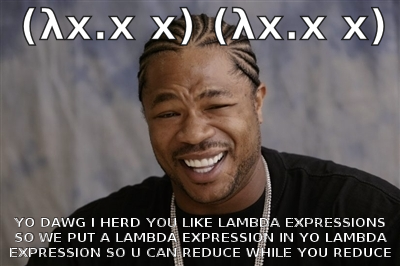
\includegraphics[width=0.7\paperwidth]{yodawg_lambda.png}
            };
        \end{tikzpicture}
    \end{blankframe}


    \section{Concluding Notes}
    \begin{frame}
        \frametitle{Further reading}
        \begin{itemize}
            \setlength{\itemsep}{1.5em}
            \item Combinatory logic (Schönfinkel 1924, Curry 1927)
            \item Curry-Howard isomorphism (Curry 1958, Howard 1969)
            \item System F (Girard 1972, Reynolds 1974)
            \item Hindley-Milner type system (Hindley 1969, Milner 1978, Damas \& Milner 1982)
        \end{itemize}
    \end{frame}

    \begin{blankframe}
        \begin{center}
            {\Huge Thank you!}
        \end{center}
    \end{blankframe}
\end{document}
